\section {Molecular Orientation}

Hydration of malonic acid by neighboring surface waters strongly affects its surface behavior. A change in the water environment around the acid can strongly alter the overall orientation of the molecule with respect to a water interface. In the following analysis we examine molecular orientation of malonic acid using a set of angles to define the molecule's orientation in space at an aqueous interface, and how the acid groups orient within in the molecule. For a complete discussion of the angles used in our analysis, we refer the reader to our previous publication that fully defines them.\cite{Blower2012}

Here we briefly introduce the angles used in the analysis, and provide a graphical depiction of their definitions in Figure \ref{fig:angle-definitions} for reference. We define the overall molecular orientation by the configuration of the three carbon atoms that form the acid's backbone. Two angles, $\theta$ and $\phi$, describe the carbon backbone ``tilt'' and ``twist'', respectively. The tilt angle, $\theta$, is measured from a reference axis (herein defined as the vector normal to the plane of the water interface) to the carbon-group bisector axis (bisecting the two C-C bonds, and pointing from the central carbon towards the direction of the other two carbon atoms). The backbone twist, $\phi$, is rotation of the carbon group about the bisector axis. If the bisector lies in the plane of the water interface such that \thetaeq 90\degr, the twist will have a value of \phieq 0\degr~when the plane of the three carbons is perpendicular to the plane of the water surface. A combination of \thetaeq 90\degr~and \phieq 90\degr~indicates an orientation with the plane of the carbon group lying flat to the plane of the water surface.

\begin{figure}[h!]
	\begin{center}
		\includegraphics[scale=1.0]{images/orientation/malonic-angle-definitions.png}
		\caption{Several angles are used to orient a malonic acid molecule both in the space-fixed frame, and internally in the molecular frame. The carbon backbone of the acid molecule has a $C_{2v}$ symmetry with a central bisector axis splitting the two C-C bonds. The bisector axis ``tilts'' relative to a fixed reference axis to form the angle $\theta$ (green). A rotation of the carbon chain group about the bisector axis changes the ``twist'' angle, $\phi$ (red). The carboxylic acid groups orient by a rotation about the two C-C bonds. The two dihedral angles, referred to as $\psi$ (blue), set the internal molecular orientation of the two carboxylic acid groups. $\psi=0$\textdegree~when a carboxylic acid is rotated such that the plane formed by the O=C-O is parallel to the plane of the three carbons, and the carbonyl C=O bond points in the direction of the carbon chain bisector. Three values of $\psi$ are depicted (right) to show how the carboxylic acid group rotates within the acid molecule.}
		\label{fig:angle-definitions}
	\end{center}
\end{figure}


Furthermore, we are able to orient the carboxylic acid moieties in the molecule by quantifying the dihedral angle, $\psi$, for each of the two acid groups. The angle $\psi$ is a rotation of the plane of the O=C-O atoms of a carboxylic acid group relative to the plane of the three carbon atoms. An orientation aligning the carbonyl bond vector (pointing from C to O) of a carboxylic acid group parallel to the carbon group bisector results in a dihedral of \psieq 0\degr. Depictions of the angle definitions, and various values of $\psi$ for one of the carboxylic acid groups, are shown in Figure \ref{fig:angle-definitions} for reference.

Plots of the \thetaphi~distributions are provided in Figure \ref{fig:theta-phi}. Three bivariate histograms are shown, depicting the orientational trends of the carbon backbone group. In these intensity plots, high intensity regions are colored darker red, and low intensity regions are colored dark blue. Regions of the plots exhibiting uniform coloration indicate isotropic behavior, whereas concentrated regions of high intensity show a preference for a particular orientation given by the specific angle combinations.

\begin{figure}[h!]
	\begin{center}
		\includegraphics[scale=1.0]{images/orientation/theta-phi.png}
		\caption{Intensity plots of the bivariate distributions of the two carbon group angles, $\theta$ and $\phi$, are plotted here. Regions of high intensity are colored red, and low intensity is colored blue. Areas of uniform coloration correspond to isotropic orientation, and small regions of intense coloration show a preference for a particular orientation. Values of $\theta$ are plotted on the horizontal, and $\phi$ is plotted on the vertical. The larger plot to the left is  a combination of results from all the simulation data. To the right are plots of the contributions from the IUB and IHB acids, on the top and bottom plots, respectively.}
		\label{fig:theta-phi}
	\end{center}
\end{figure}


The larger plot on the left of Figure \ref{fig:theta-phi} shows the distribution collected from the data of all five simulations. The highest intensity region is centered at \thetaeq 135\degr, and \phieq 90\degr. This indicates an orientation of the plane of the carbon backbone group tilted 45\degr~from the plane of the water surface with the central carbon further out towards the gas-phase side of the interface than the two carbonyl carbons. Additionally, the $\phi$ values show that the two carbonyl carbons are both at similar depths into the water side of the interface.

Although the entire range of $\theta$ and $\phi$ values are found in the distribution, the bulk of the intensity is concentrated around \thetaeq 135\degr, and very little appears in the region below \thetaeq 90\degr. Thus, there is a clear orientational preference established for the carbon group atoms, and this has a direct effect on the orientation of the other atoms in the molecule.

These orientational results complement those found in our previous classical force field simulation study of malonic acid.\cite{Blower2012} In that study the behavior of the top-most malonic acid molecules on a water surface exhibited a very similar \thetaphi~distribution as in the results shown in Figure \ref{fig:theta-phi}. However, in the classical simulations, acids located deeper into the water bulk reoriented, resulting in interfacial layering of orientational preferences that changed with depth. In the present work, none of the simulated molecules moved into the water side of the interface (i.e. penetrated the water bulk). Likely, this is because of the length of the simulations and the system geometry. Hence, only the top-most acids on a water surface are represented in the simulations, and comparison with the results from the previous classical simulations are limited, accordingly.

The results of the \thetaphi~analysis were further broken down to differentiate between IUB and IHB systems. These are plotted on the top-right and bottom-right of Figure \ref{fig:theta-phi}, respectively. IUB systems exhibit a very strong orientational preference in $\theta$. The IUB set of acids are entirely oriented with $\theta >$ 90\degr, and the distribution is tightly concentrated around \thetaeq 135\degr. The twist, $\phi$, is concentrated around a value of approximately \phieq 75\degr, with a smaller high-intensity region at $\phi >$ 80\degr. As the twist angle decreases from 90\degr~the two ends of the carbon atom chain move to different depths in the interface. Upper values of $\phi$ in the most intense region of the distribution reach near \phieq 60\degr, resulting from a twist that sends one end of the molecule 30\degr~further out of the aqueous surface than the other. The IUB acids are thus more likely to experience different solvation environments at either end of the molecule if one end is further away from surface waters.

Turning now to the IHB malonic acid \thetaphi~plot of Figure \ref{fig:theta-phi}, we see slightly different orientational preferences. The region of highest intensity is concentrated at \phieq 90\degr, but spread over a wide range of $\theta$, approximately between 90\degr $< \theta <$150\degr. Furthermore, $\theta$ values in the plot span the entire range down to \thetaeq 0\degr. Clearly the intramolecular bonding leads to greater orientational freedom of the carbon backbone as evidenced by the less concentrated distribution and greater range of orientations. This is intuitively expected for a molecule that has less bonding to neighboring waters due to an internal hydrogen bond partially occupying both carboxylic acid functional groups. Water is less likely to interact with a malonic acid that has fewer binding sites, and will not stabilize the acid's position or orientation as strongly as it would in the IUB molecule. Thus, the internal H-bond gives the acid molecule access to many more orientations on the water surface than its counterpart: the IUB acid.

The internal geometry of malonic acid is defined here by the two dihedral angles that quantify rotations of the carboxylic acid groups about the molecule's two C-C bonds. As mentioned earlier, the angle $\psi$ is referenced by the alignment of the C=O carbonyl bond with the C-C-C group bisector. Figure \ref{fig:angle-definitions} depicts various orientations of a carboxylic acid group and the accompanying values of $\psi$. The overall \psipsi~distribution is plotted on the left of Figure \ref{fig:psi-psi} with the plots of the IUB and IHB systems to the right in the figure on top and bottom, respectively. We do not distinguish here between the two carboxylic acid groups of the acid molecules. Consequently, the horizontal and vertical axes of the \psipsi~plots are arbitrarily assigned to one of the two acid dihedral angles. The larger plot of all simulation data is overwhelmed by the high intensity concentration at the \psipsi~region of 0\degr-180\degr~at the bottom left of the plot. Much lower intensity regions appear throughout the \psipsi~range.


\begin{figure}[h!]
	\begin{center}
		\includegraphics[scale=1.0]{images/orientation/psi-psi.png}
		\caption{Intensity plots of the bivariate $\psi$-$\psi$ distribution of the two dihedral angles are plotted here, arranged and colored in the same manner as the $\theta$-$\phi$ distributions of Figure \ref{fig:theta-phi}.} 
		\label{fig:psi-psi}
	\end{center}
\end{figure}

Looking to the IHB plot at the bottom right of Figure \ref{fig:psi-psi} it is clear why the larger plot of all the data sets is similarly concentrated at the bottom left of the plot. All of the intensity of the IHB acids indicates that the two carbonyl C=O bonds are aligned anti-parallel to each other. The strong H-bond holds the internal geometry nearly fixed with very little distortion through bending of the acid's six-member atom ring structure, or twisting of the carboxylic acids around the C-C bonds. An intense and highly concentrated region of the dihedral angle distribution is indicative of a stable, virtually rigid form of the IHB malonic acid.

The IUB malonic acids exhibit a very different behavior in their carboxylic acid orientations. The top-right plot of Figure \ref{fig:psi-psi} shows the much broader, less concentrated distribution resulting from acids without the internal H-bonding constraints. The broad regions of low intensity throughout the distribution demonstrates the molecule's much greater flexibility, a consequence of having the two carboxylic acid ends of the molecule much more decoupled. However, a trend is apparent in the distribution of the two dihedral angles. Note the two regions of intensity in the plot located at the center-left and top-center. In our previously published results of the complementary classical interaction potential simulations,\cite{Blower2012} the \psipsi~distributions throughout the interfacial region had two similarly located regions. In that study the regions of the plot were more concentrated over small areas at \psipsi~values of 0\degr~and 90\degr. That combination is indicative of the dihedrals aligning 90\degr~from each other, i.e. perpendicularly. One of the C=O bonds is aligned parallel to the C-C-C bisector (\psieq 0\degr), and the other is perpendicular to the plane formed by the C-C-C atoms (\psieq 90\degr). The correspondence of the two regions in the distribution of the present work to those of the classical simulations is noteworthy. The classical force field reproduces the dihedral trend of two peaks in the distribution, but the much smaller range of $\psi$ angles suggests that the corresponding dihedral term in the classical potential needs to be adjusted to better recreate the KS-DFT results for higher accuracy. The present results, however, demonstrate that without further modifications, there is reasonable agreement between the KS-DFT and classical interaction potentials with regards to the overall orientation of surface malonic acid molecules. The shortcoming of the classical interaction potential is its inability to properly capture the IHB conformation. However, that conformation may not be a major contributor to the distribution of acids found at a water surface.

% theta_{C=O}
Having now established the \thetaphi~orientational trend of the carbon backbone atoms, and the \psipsi~dihedral relationships, we have a nearly complete orientational picture of malonic acid on a water surface. What remains is to determine the absolute orientation of both carboxylic acid groups with respect to the plane of the water surface. In order to compare the computed orientational results with our recent experimental results,\cite{Blower2012} determined by the SFG spectra of the carbonyl modes of malonic acid, we now discuss further the configuration of the carboxylic acid groups. Specifically, the analysis presented shows how the carbonyl C=O bond vectors orient relative to the reference axis normal to the plane of the interface, forming a carbonyl tilt angle, \thetacarb.

The distribution of \thetacarb~is presented in Figure \ref{fig:theta-carb}. The black plot shows the distribution of angles from all simulation datasets. The red and blue plots correspond to the \thetacarb~data collected only from the IHB, and IUB simulations, respectively. In all the distributions two angle regions dominate in intensity, appearing as peaks from approximately 50\degr-120\degr, and 150\degr-180\degr. The former angle range corresponds to carbonyl C=O bonds pointing in the plane of the water surface ($\theta_{C=O}=90$\degr~indicates a carbonyl parallel to the plane), slightly above, or slightly below the plane. The latter range indicates carbonyl bonds pointing directly in towards the water side of the interface ($\theta_{C=O}=180$\degr) or within a cone of approximately 30\degr~tilt from the reference axis into the water bulk.

\begin{figure}[h!]
	\begin{center}
		\includegraphics[scale=1.0]{images/orientation/ThetaCarbonyl.png}
		\caption{The tilt angle, \thetacarb, of the two carbonyl C=O bonds of malonic acid were calculated throughout each simulation. The \thetacarb~angle distributions were then calculated and are shown here for all simulations (black), for IUB simulations (blue) and for the IHB simulations (red).}
		\label{fig:theta-carb}
	\end{center}
\end{figure}

Looking at the individual red and blue plots, there are some differences between how the internal bonding conformations behave. The lower peak of the blue plot is centered at approximately $\theta_{C=O}=90$\degr, extending up to 30\degr~to either side. The peak near 180\degr~extends down to 130\degr. Between the two peaks there is a small intensity, whereas for $\theta_{C=O} < 50$\degr, there is no intensity as the distribution drops to zero. 

The red plot, representing the IHB acids, is lower in overall magnitude than the blue plot because only two of the five simulations are represented. Additionally, there is intensity throughout the entire \thetacarb~range, as compared to the blue plot that loses intensity at the lower angles. The location of the lower red peak is centered near $\theta_{C=O}=70$\degr, which is almost 20\degr~lower than the equivalent blue distribution peak. The width of the red peak is smaller, narrower by approximately 20\degr. The peak at 180\degr~similarly narrows by nearly 20\degr.

In both sets of simulations there is a clear trend for malonic acid to point one of its carbonyl bonds into the water side of the interface ($\theta_{C=O}=180$\degr), and the other bond points in the plane of the interface, or slightly above of below it ($\theta_{C=O} \approx 90$\degr). The formation of the internal H-bond slightly shifts the angle of the in-plane carbonyl to point further out away from the water side of the interface ($\theta_{C=O} \approx 70$\degr). Also, the IHB acids enjoy a greater orientational freedom in their carbonyls overall (i.e. the distribution has intensity throughout all angle regions), but the peaks in the distribution are narrower than for the IUB molecules. It is likely that the orientation of the carbonyl bonds on the water surface is affected by their solvation environments, and hydration by surface waters. The IHB malonic acid has a peak in the distribution of \thetacarb~that lies slightly further to the left (i.e. lower angle values) than its unbonded counterpart. Lower angle values indicate a carbonyl bond tilt further out from the surface, away from the water bulk. This slight orientational difference likely leads to a difference in the strength, or amount of hydration on this particular carbonyl bond. The effect of this will become apparent spectrally, and may lead to interesting chemical differences between the two conformations.
